\chapter{Results}%Or Results
\label{ch:res}
Let us start drawing a big picture of the different topics that emerged after the latent ideology analysis. 


Fig \ref{fig:diptest} summarizes the size of the networks and the diptest results -the polarization- for each topic. The first thing to note is the fact that  the highest polarization corresponds to the smaller topics, with the exception of topic 14; For the first two topics the polarization is significantly higher than the others. The average diptest score for COP26 is $0.069$.


\begin{figure}[H]
    \centering
    \includegraphics[width=0.95\linewidth]{Chapter5//figures/dip_test_cop26.pdf}
    \caption{Dip test and number of users for cop26 topic by topic}
    \label{fig:diptest}
\end{figure}

\section{RQ1 Most Polarized Topics}


Fig \ref{fig:networks_polarization} demonstrates the most and the least polarized topics. Every network represents the retweet network of the 100 biggest influencers; in the leftmost plots there is the full network, while in the rightmost only the influencers are present. In the most polarized topics it can be clearly seen how the influencers are almost equally split between the two poles. 
Falkenberg, in his work, identified a majority of pro climate users and a minority of climate skeptics but, looking at a topic level, the two groups are equally split and the networks that present the majority-minority dichotomy are the least polarized. A notable example is topic 34: "Canada Climate Change goals", which refers to the decision of Canada’s prime minister to cap gas and oil emissions. 
This announcement caused much disagreement, displayed in Tab \ref{tab:canadatweets} with some random tweets against the decision, User1’s argument is that this will destroy the economy; while User2 is instead generally against all the decision of Trudeau, as stated in her biography : "Lover of gardening, antiques and anyone who wants to see the end of the Trudeau government." This follows the typical elite polarization pattern, where political exponents strictly adhere to their party policies. In this case, it is not a political party but a politically-aligned individual, which is, in some way, forced to follow her self-imposed guidelines in her biography to avoid cognitive dissonance  \cite{Festinger_dissonance_57}. Looking at the right side of \ref{fig:networks_polarization} we can see how the influencers, whom we can use as a proxy to the elite, tend to be more polarized than the ’mass’. This is especially evident in topic 14, related to air travel, where the influencers are lined up, while the normal users are more distributed in the spectrum.


\begin{table}[]
\centering
\begin{tabular}{|p{1in}|p{4in}|}\hline
\textbf{user} & \textbf{tweet} \\ \hline
User1     & This meme could just as easily apply to Canada. Trudeau’s willingness to destroy our economy to the benefit of others is akin to cutting off our noses to spite our faces!\%. \\ \hline
User2        & \#COP26 Maybe some people are still fooled by Justin Trudeau and his dishonest climate change stories, but there are plenty of us here in Canada who are not. Look into the truth about the Lytton fire. It won't come out of Justin Trudeau's mouth \\ \hline
User3          & Capping emissions in the country while exporting oil, gas and coal out of the country. Hypocrisy.
 \\ \hline
\end{tabular}
\caption{}
\label{tab:canadatweets}
\end{table}




It is interesting to note in Fig \ref{fig:ridge_topics} the distribution of the tweets of each topic over time during the COP, with the dotted line marking the start and end date of COP26. The most polarized had interest only  for a few days, quickly losing  interest. The opposite happens in the least polarized topics where the discussion is distributed over a longer timespan.



\begin{figure}[H]
    \centering
    \begin{minipage}{0.50\textwidth}
        \centering
         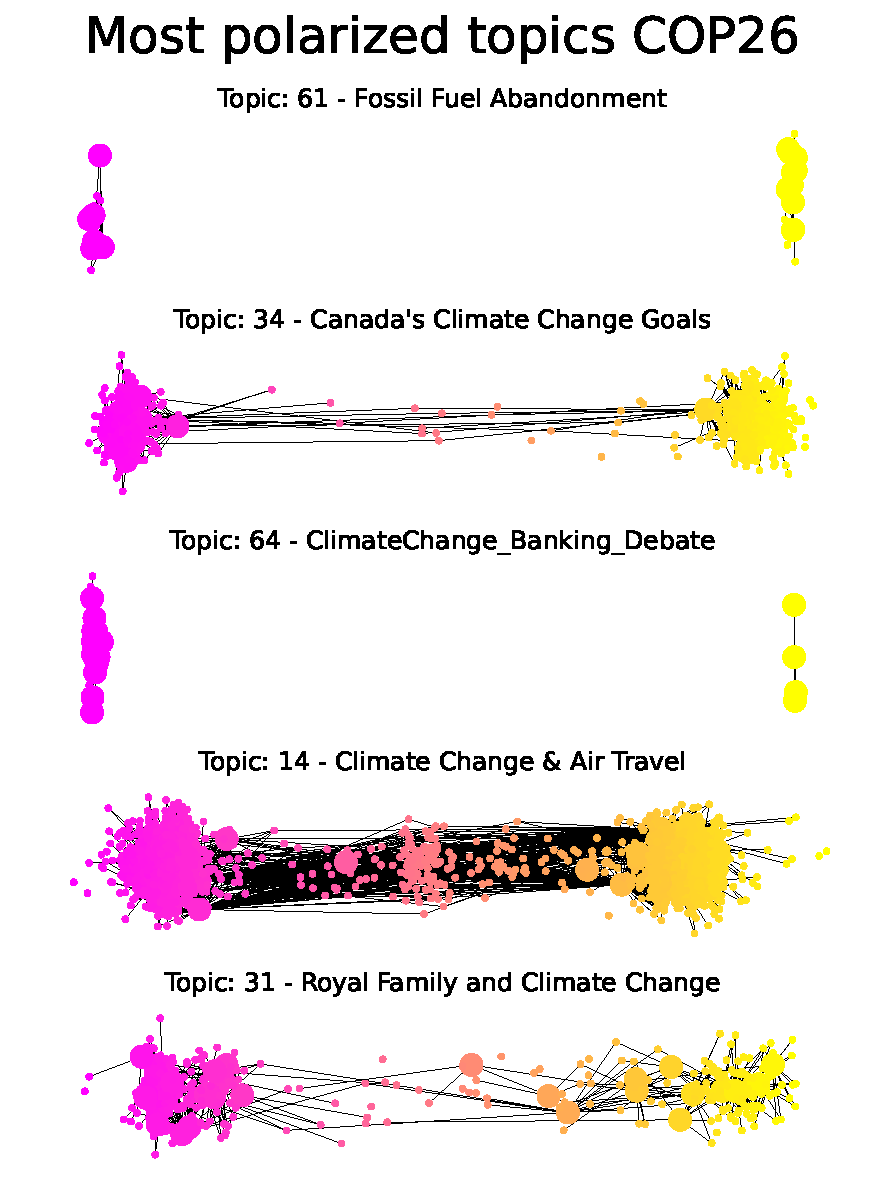
\includegraphics[width=0.98\linewidth]{Chapter5/figures/Most polarized topics COP26.pdf}
        
    \end{minipage}\hfill
    \begin{minipage}{0.50\textwidth}
        \centering
         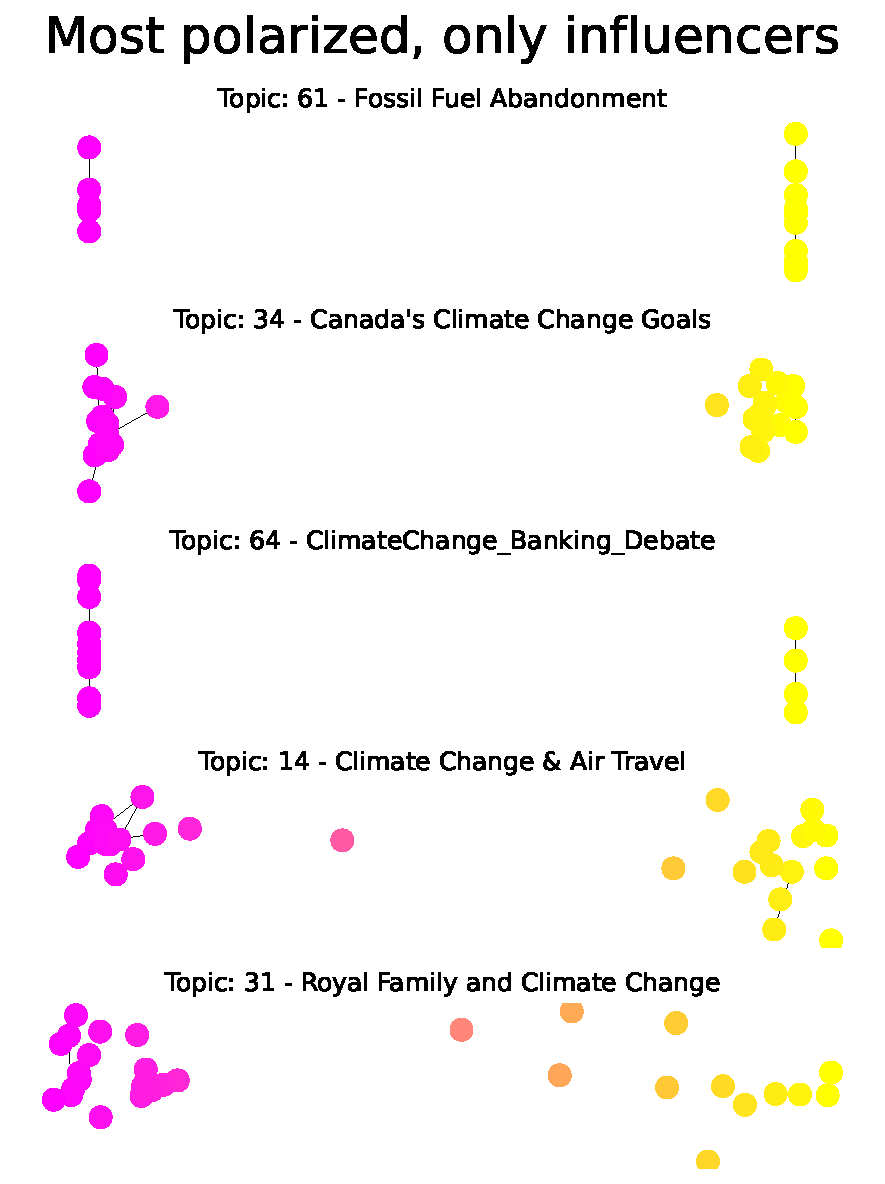
\includegraphics[width=0.98\linewidth]{Chapter5/figures/Most polarized, only influencers.pdf}
        
    \end{minipage}
    \begin{minipage}{0.50\textwidth}
        \centering
         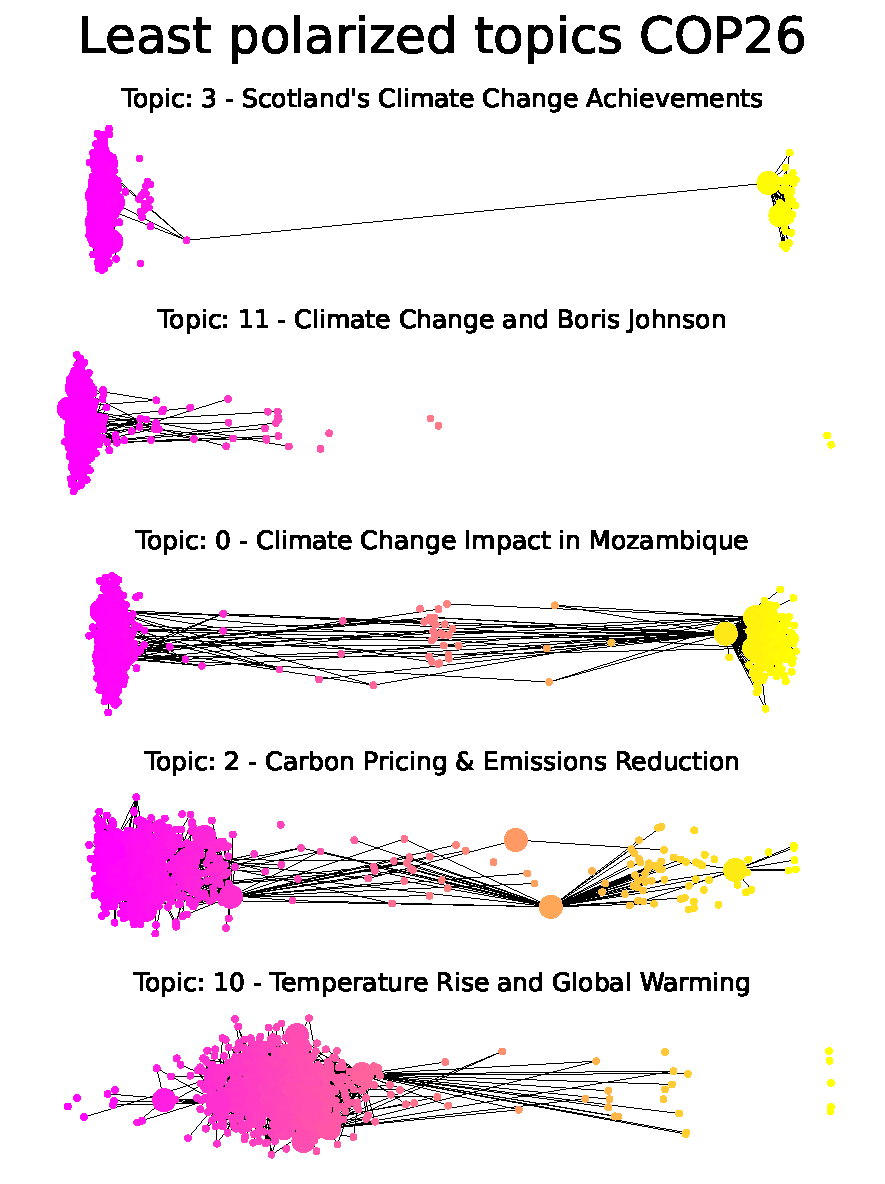
\includegraphics[width=0.98\linewidth]{Chapter5/figures/Least polarized topics COP26.pdf}
        
    \end{minipage}\hfill
    \begin{minipage}{0.50\textwidth}
        \centering
         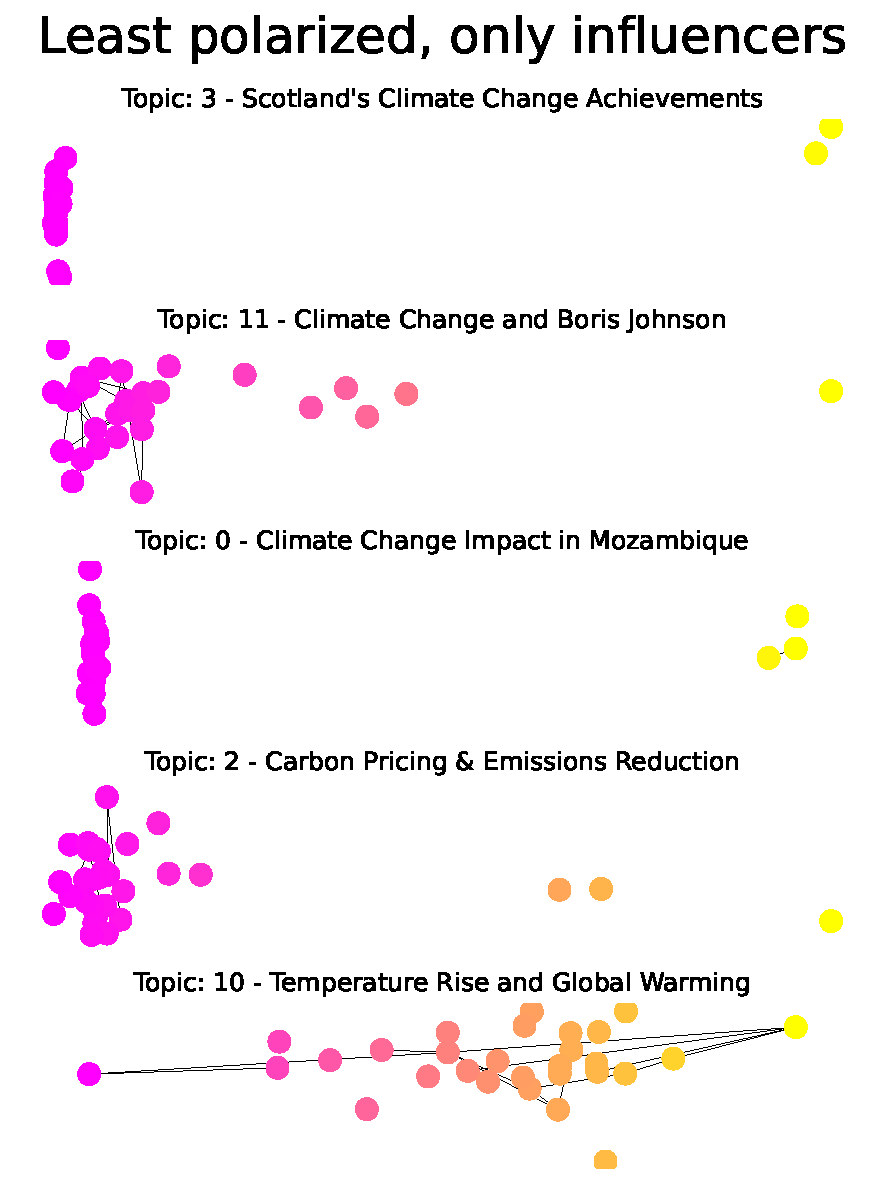
\includegraphics[width=0.98\linewidth]{Chapter5/figures/Least polarized, only influencers.pdf}
        
    \end{minipage}

    \caption{Most and Least polarized topics in cop 26; on the right side the full network, on the left side the influencers network.}
    \label{fig:networks_polarization}
\end{figure}


\begin{figure}[H]
    \centering
    \begin{minipage}{0.50\textwidth}
        \centering
         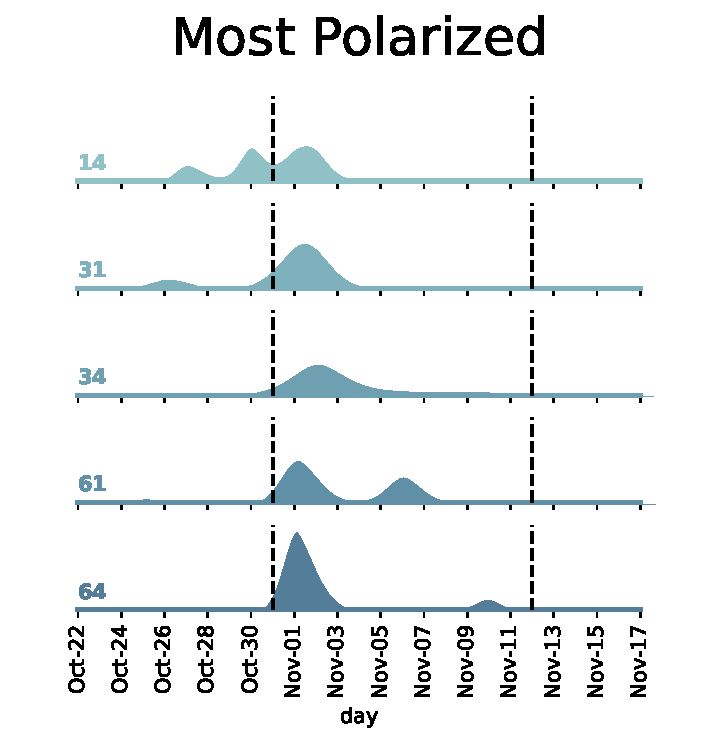
\includegraphics[width=0.98\linewidth]{Chapter5/figures/ridge_most.pdf}
        
    \end{minipage}\hfill
    \begin{minipage}{0.50\textwidth}
        \centering
         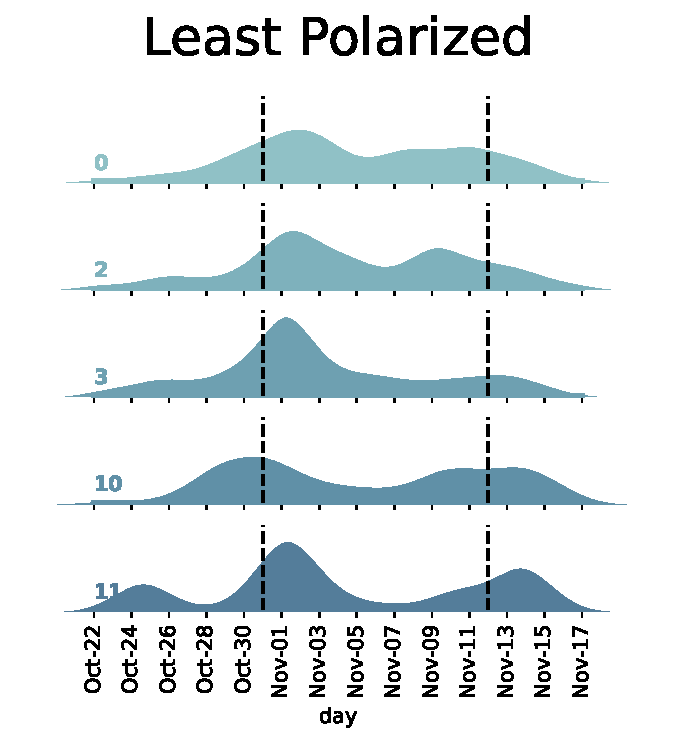
\includegraphics[width=0.98\linewidth]{Chapter5/figures/ridge_least.pdf}
        
    \end{minipage}

    \caption{ Distribution of tweets belonging to the most and least polarized topics during the days around COP26}
    \label{fig:ridge_topics}
\end{figure}


\section{RQ2 Longitudinal analysis}

In this section a comparison is made about  the polarization between COP21 and COP26 and, to do so, it was necessary to run the topic modeling together. In Fig \ref{fig:diptesto cop2x} the diptest results are shown, and a similar trend to that of the cop26 is evident: the biggest topics are less polarized, with the exception of topic 9. Fig \ref{fig:2126_share} helps understand the share of the tweets between cop21 and COP26. It is also interesting to see that topic 9, which is the most polarized, is composed mostly by tweets from COP26, being therefore aligned with the literature. Now the focus of this work will shift to some topics, creating the network of retweets for both COPs, which will then be compared. The computation of this analysis is possible only for topic 1,3 and 12, which are the ones that are polarized and have enough tweets in both cops to run latent ideology.


\begin{figure}[H]
    \centering
    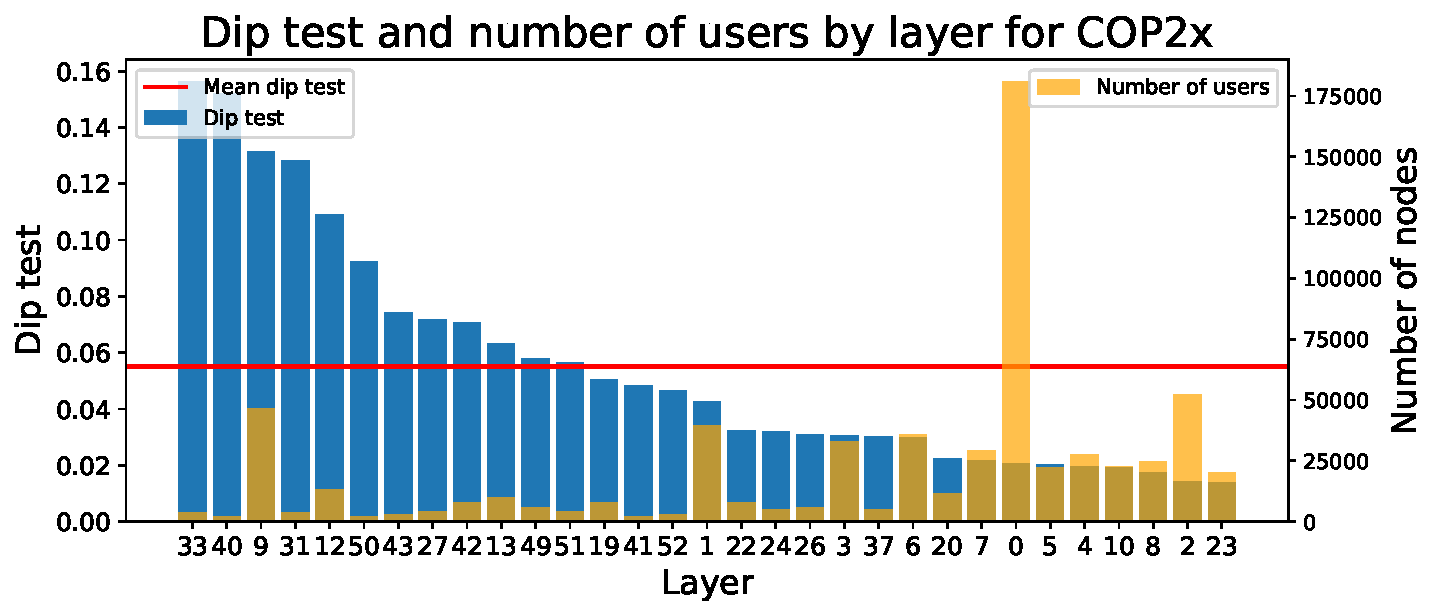
\includegraphics[width=0.99\linewidth]{Chapter5//figures/dip_test_COP2x.pdf}
    \caption{Dip test result for COP2x, containing both tweets of COP21 and COP26}
    \label{fig:diptesto cop2x}
\end{figure}

\begin{figure}[H]
    \centering
    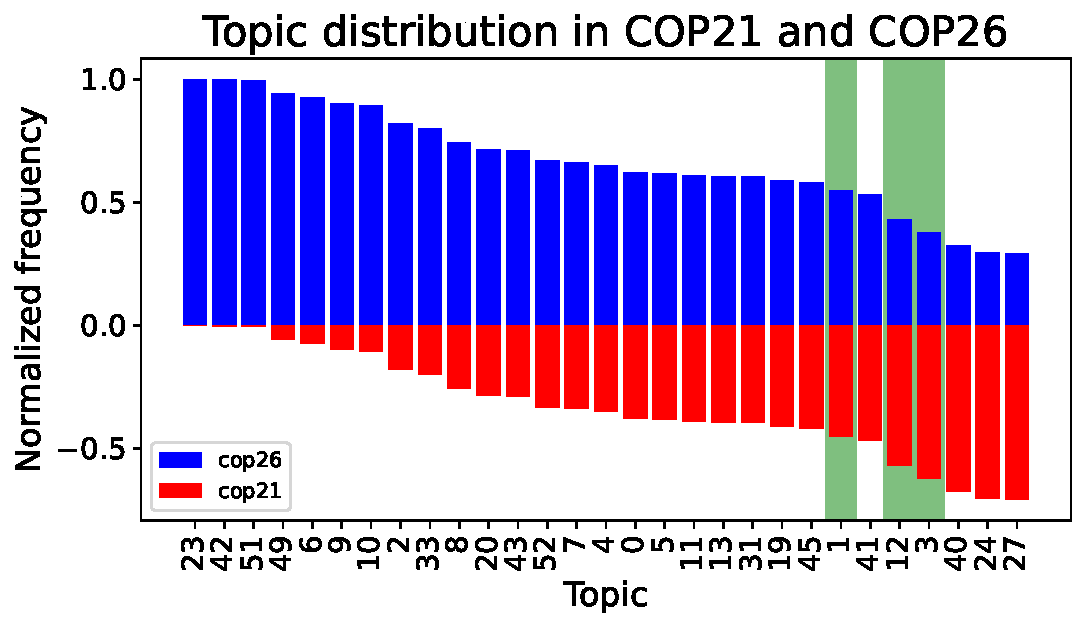
\includegraphics[width=0.9\linewidth]{Chapter5/figures/2x_topic_distribution.pdf}
    \caption{The share of the tweets, topic by topic, between COP21 and COP26 }
    \label{fig:2126_share}
\end{figure}

Fig \ref{fig:cop2x_network_comparison}  shows the results of this analysis. It is worth noting how topic 12 is the topic dealing with Canadian fossil fuels, discussion that was present in both COPs, but with a very different level of polarization. Overall, the results confirm the hypothesis that COP26 is more polarized than COP21, but these are just three topics, thus the same analysis with more data should be run to confirm it.

\begin{figure}[H]
    \centering
    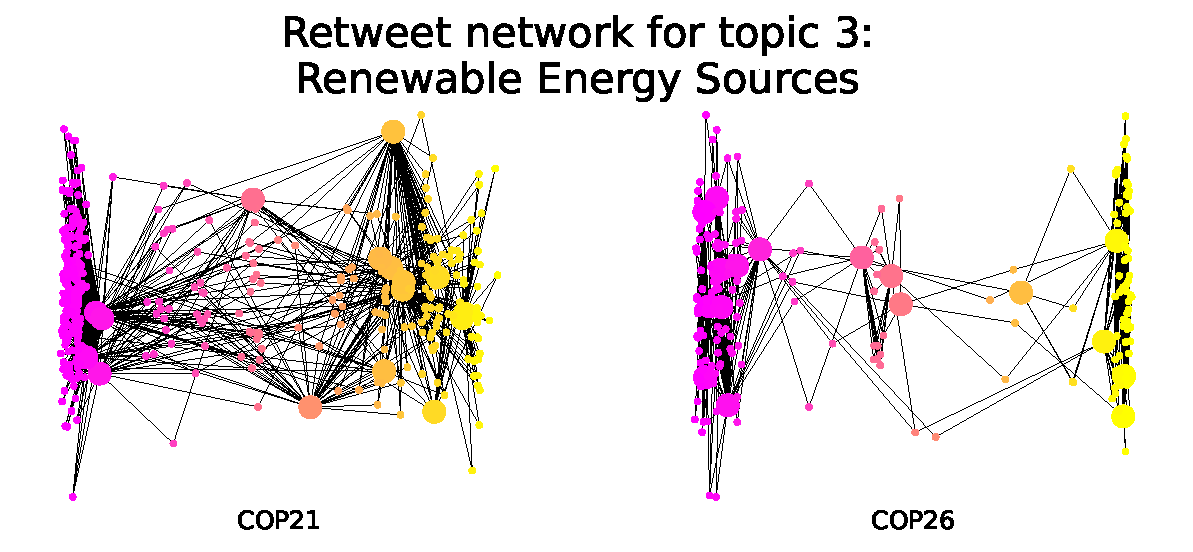
\includegraphics[width=0.95\linewidth]{Chapter5/figures/2x_topic3_network.pdf}
    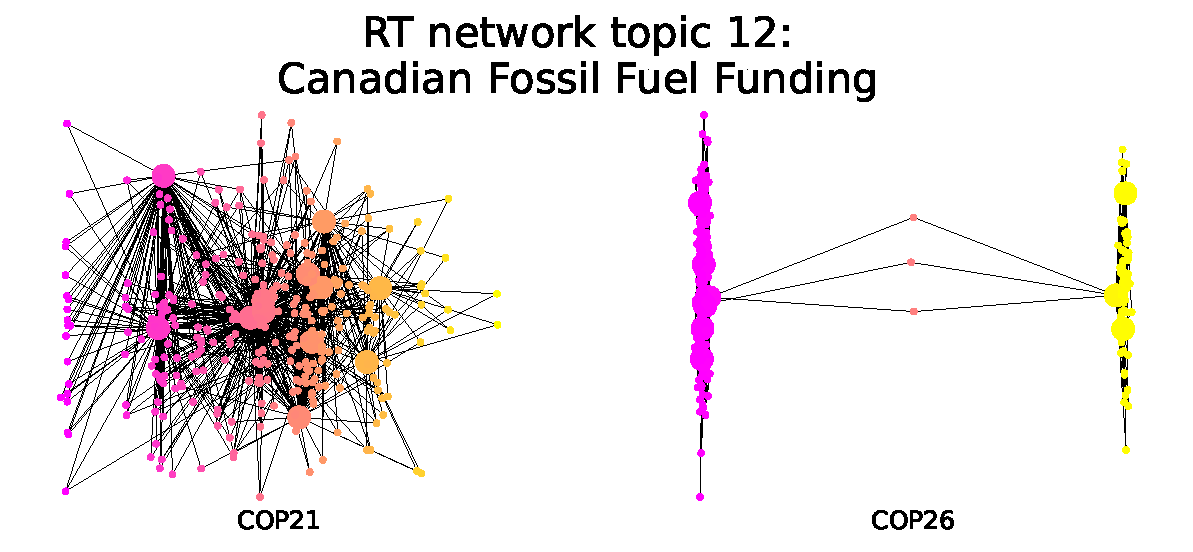
\includegraphics[width=0.95\linewidth]{Chapter5/figures/2x_topic12_network.pdf}
    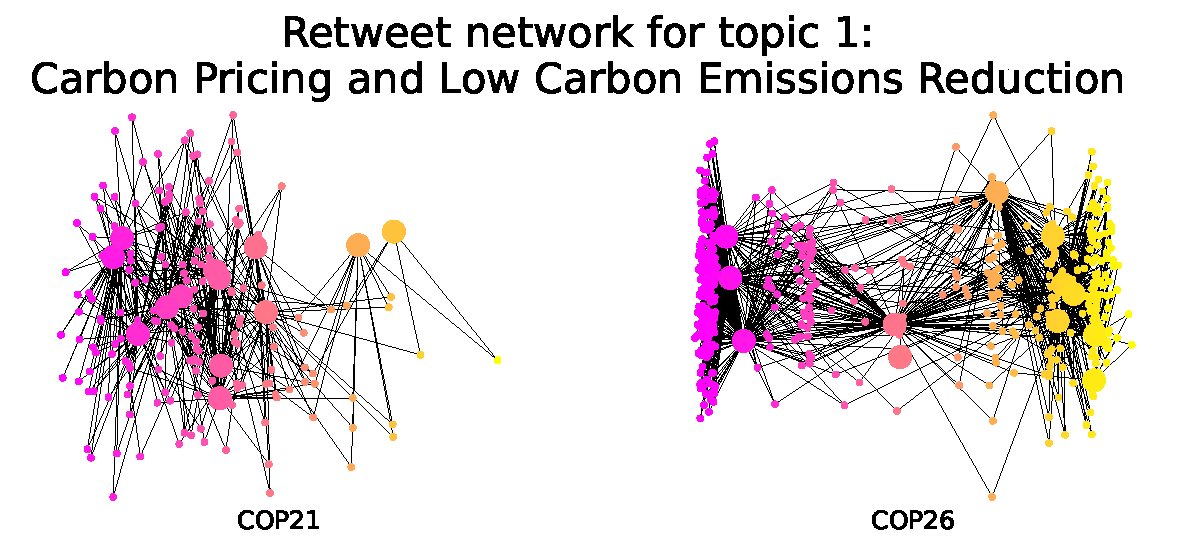
\includegraphics[width=0.95\linewidth]{Chapter5/figures/2x_topic1_network.pdf}
    \caption{A comparison of the retweet network about the same topic for COP21 and COP26}
    \label{fig:cop2x_network_comparison}
\end{figure}

\section{RQ3 User polarization among different topics}
After computing the polarization score for all users, it can now be analyzed whether the users are polarized in the same way among all the topics they were active in.

The number of users involved in this analysis is 22161, active in 26 topics. Most of them (16141) were only active in one topic, while the maximum is 23, and the average is 1.53 topics per user.

Then, the average and the standard deviation of the score was computed for each user present in more than 1 topic. This value is higher for the users that are present in both sides of the spectrum, allowing for the identification of the degree to which users tend to be monopolar.


Fig \ref{fig:std_avg} shows how the distribution of the average score for every topic aggregated together.
 This matches the global results of Falkenberg, where a majority is present on the $−1$ side versus a minority in the $1$ side.


In the distribution of the std(standard deviation) we can see how there is a strong tendency to stay in the same side of the spectrum.

\begin{figure}[H]
    \centering
    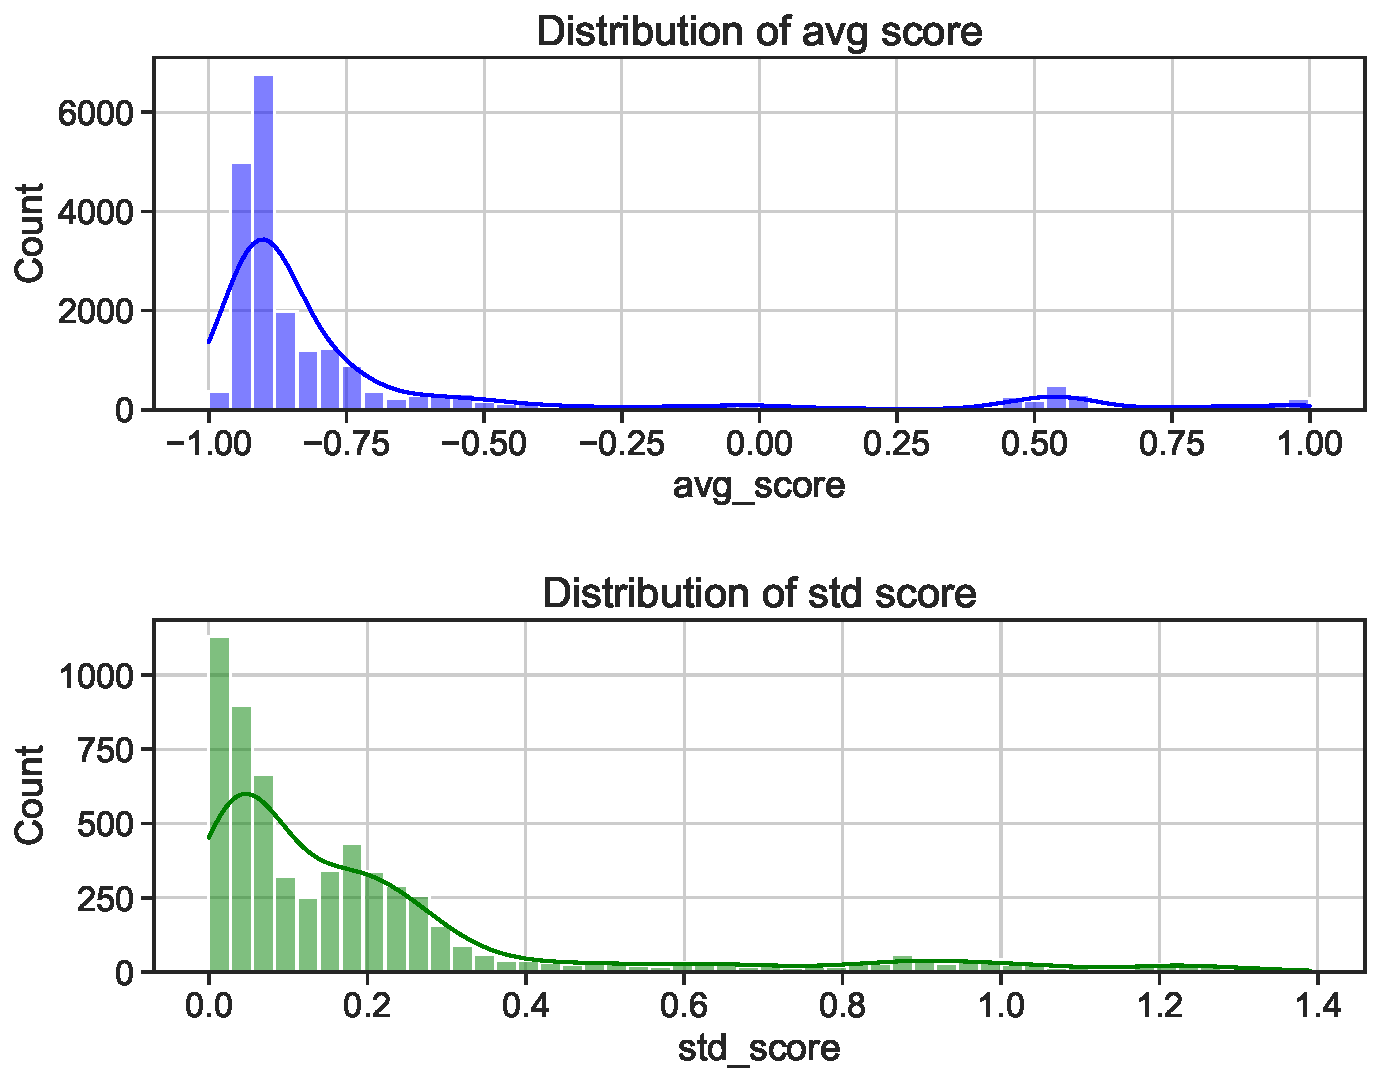
\includegraphics[width=0.9\linewidth]{Chapter5/figures/avg_std_score.pdf}
    
    \caption{distribution of the mean and the standard deviation of users' score}
    \label{fig:std_avg}
\end{figure}



\section{RQ4 Polarization of mono vs poli topic users }
Out of the 22 thousand users, most of them (16 thousand) are present only in one topic; out of the 6000 present in more than one topic, half of them are present in only 2. Fig \ref{fig:monopoli} does not show a big difference in the ideology score between mono and poli users (0.8 for monotopic users, 0.82 for politopic). The computation of this score considered only the absolute value.


\begin{figure}
    \centering
    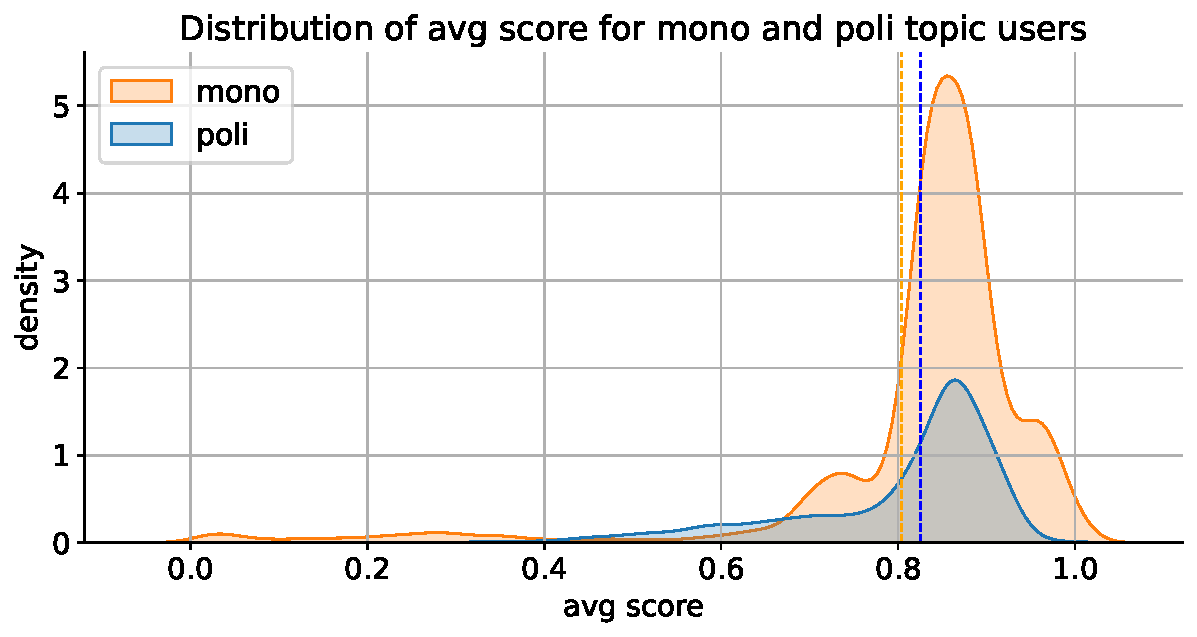
\includegraphics[width=0.8\linewidth]{Chapter5/figures/avg_score_mono_poli.pdf}
    \caption{A comparison of the absolute value of the average score both for users that are present in one topic(mono) and on multiple (poli)}
    \label{fig:monopoli}
\end{figure}

